\documentclass{ximera}

%\usepackage{todonotes}

\newcommand{\todo}{}

\usepackage{esint} % for \oiint
\ifxake%%https://math.meta.stackexchange.com/questions/9973/how-do-you-render-a-closed-surface-double-integral
\renewcommand{\oiint}{{\large\bigcirc}\kern-1.56em\iint}
\fi


\graphicspath{
  {./}
  {ximeraTutorial/}
  {basicPhilosophy/}
  {functionsOfSeveralVariables/}
  {normalVectors/}
  {lagrangeMultipliers/}
  {vectorFields/}
  {greensTheorem/}
  {shapeOfThingsToCome/}
  {dotProducts/}
  {../productAndQuotientRules/exercises/}
  {../normalVectors/exercisesParametricPlots/}
  {../continuityOfFunctionsOfSeveralVariables/exercises/}
  {../partialDerivatives/exercises/}
  {../chainRuleForFunctionsOfSeveralVariables/exercises/}
  {../commonCoordinates/exercisesCylindricalCoordinates/}
  {../commonCoordinates/exercisesSphericalCoordinates/}
  {../greensTheorem/exercisesCurlAndLineIntegrals/}
  {../greensTheorem/exercisesDivergenceAndLineIntegrals/}
  {../shapeOfThingsToCome/exercisesDivergenceTheorem/}
  {../greensTheorem/}
  {../shapeOfThingsToCome/}
}

\newcommand{\mooculus}{\textsf{\textbf{MOOC}\textnormal{\textsf{ULUS}}}}

\usepackage{tkz-euclide}\usepackage{tikz}
\usepackage{tikz-cd}
\usetikzlibrary{arrows}
\tikzset{>=stealth,commutative diagrams/.cd,
  arrow style=tikz,diagrams={>=stealth}} %% cool arrow head
\tikzset{shorten <>/.style={ shorten >=#1, shorten <=#1 } } %% allows shorter vectors

\usetikzlibrary{backgrounds} %% for boxes around graphs
\usetikzlibrary{shapes,positioning}  %% Clouds and stars
\usetikzlibrary{matrix} %% for matrix
\usepgfplotslibrary{polar} %% for polar plots
\usepgfplotslibrary{fillbetween} %% to shade area between curves in TikZ
\usetkzobj{all}
%\usepackage[makeroom]{cancel} %% for strike outs
%\usepackage{mathtools} %% for pretty underbrace % Breaks Ximera
%\usepackage{multicol}
\usepackage{pgffor} %% required for integral for loops



%% http://tex.stackexchange.com/questions/66490/drawing-a-tikz-arc-specifying-the-center
%% Draws beach ball
\tikzset{pics/carc/.style args={#1:#2:#3}{code={\draw[pic actions] (#1:#3) arc(#1:#2:#3);}}}



\usepackage{array}
\setlength{\extrarowheight}{+.1cm}   
\newdimen\digitwidth
\settowidth\digitwidth{9}
\def\divrule#1#2{
\noalign{\moveright#1\digitwidth
\vbox{\hrule width#2\digitwidth}}}





\newcommand{\RR}{\mathbb R}
\newcommand{\R}{\mathbb R}
\newcommand{\N}{\mathbb N}
\newcommand{\Z}{\mathbb Z}

\newcommand{\sagemath}{\textsf{SageMath}}


%\renewcommand{\d}{\,d\!}
\renewcommand{\d}{\mathop{}\!d}
\newcommand{\dd}[2][]{\frac{\d #1}{\d #2}}
\newcommand{\pp}[2][]{\frac{\partial #1}{\partial #2}}
\renewcommand{\l}{\ell}
\newcommand{\ddx}{\frac{d}{\d x}}

\newcommand{\zeroOverZero}{\ensuremath{\boldsymbol{\tfrac{0}{0}}}}
\newcommand{\inftyOverInfty}{\ensuremath{\boldsymbol{\tfrac{\infty}{\infty}}}}
\newcommand{\zeroOverInfty}{\ensuremath{\boldsymbol{\tfrac{0}{\infty}}}}
\newcommand{\zeroTimesInfty}{\ensuremath{\small\boldsymbol{0\cdot \infty}}}
\newcommand{\inftyMinusInfty}{\ensuremath{\small\boldsymbol{\infty - \infty}}}
\newcommand{\oneToInfty}{\ensuremath{\boldsymbol{1^\infty}}}
\newcommand{\zeroToZero}{\ensuremath{\boldsymbol{0^0}}}
\newcommand{\inftyToZero}{\ensuremath{\boldsymbol{\infty^0}}}



\newcommand{\numOverZero}{\ensuremath{\boldsymbol{\tfrac{\#}{0}}}}
\newcommand{\dfn}{\textbf}
%\newcommand{\unit}{\,\mathrm}
\newcommand{\unit}{\mathop{}\!\mathrm}
\newcommand{\eval}[1]{\bigg[ #1 \bigg]}
\newcommand{\seq}[1]{\left( #1 \right)}
\renewcommand{\epsilon}{\varepsilon}
\renewcommand{\phi}{\varphi}


\renewcommand{\iff}{\Leftrightarrow}

\DeclareMathOperator{\arccot}{arccot}
\DeclareMathOperator{\arcsec}{arcsec}
\DeclareMathOperator{\arccsc}{arccsc}
\DeclareMathOperator{\si}{Si}
\DeclareMathOperator{\scal}{scal}
\DeclareMathOperator{\sign}{sign}


%% \newcommand{\tightoverset}[2]{% for arrow vec
%%   \mathop{#2}\limits^{\vbox to -.5ex{\kern-0.75ex\hbox{$#1$}\vss}}}
\newcommand{\arrowvec}[1]{{\overset{\rightharpoonup}{#1}}}
%\renewcommand{\vec}[1]{\arrowvec{\mathbf{#1}}}
\renewcommand{\vec}[1]{{\overset{\boldsymbol{\rightharpoonup}}{\mathbf{#1}}}}
\DeclareMathOperator{\proj}{\vec{proj}}
\newcommand{\veci}{{\boldsymbol{\hat{\imath}}}}
\newcommand{\vecj}{{\boldsymbol{\hat{\jmath}}}}
\newcommand{\veck}{{\boldsymbol{\hat{k}}}}
\newcommand{\vecl}{\vec{\boldsymbol{\l}}}
\newcommand{\uvec}[1]{\mathbf{\hat{#1}}}
\newcommand{\utan}{\mathbf{\hat{t}}}
\newcommand{\unormal}{\mathbf{\hat{n}}}
\newcommand{\ubinormal}{\mathbf{\hat{b}}}

\newcommand{\dotp}{\bullet}
\newcommand{\cross}{\boldsymbol\times}
\newcommand{\grad}{\boldsymbol\nabla}
\newcommand{\divergence}{\grad\dotp}
\newcommand{\curl}{\grad\cross}
%\DeclareMathOperator{\divergence}{divergence}
%\DeclareMathOperator{\curl}[1]{\grad\cross #1}
\newcommand{\lto}{\mathop{\longrightarrow\,}\limits}

\renewcommand{\bar}{\overline}

\colorlet{textColor}{black} 
\colorlet{background}{white}
\colorlet{penColor}{blue!50!black} % Color of a curve in a plot
\colorlet{penColor2}{red!50!black}% Color of a curve in a plot
\colorlet{penColor3}{red!50!blue} % Color of a curve in a plot
\colorlet{penColor4}{green!50!black} % Color of a curve in a plot
\colorlet{penColor5}{orange!80!black} % Color of a curve in a plot
\colorlet{penColor6}{yellow!70!black} % Color of a curve in a plot
\colorlet{fill1}{penColor!20} % Color of fill in a plot
\colorlet{fill2}{penColor2!20} % Color of fill in a plot
\colorlet{fillp}{fill1} % Color of positive area
\colorlet{filln}{penColor2!20} % Color of negative area
\colorlet{fill3}{penColor3!20} % Fill
\colorlet{fill4}{penColor4!20} % Fill
\colorlet{fill5}{penColor5!20} % Fill
\colorlet{gridColor}{gray!50} % Color of grid in a plot

\newcommand{\surfaceColor}{violet}
\newcommand{\surfaceColorTwo}{redyellow}
\newcommand{\sliceColor}{greenyellow}




\pgfmathdeclarefunction{gauss}{2}{% gives gaussian
  \pgfmathparse{1/(#2*sqrt(2*pi))*exp(-((x-#1)^2)/(2*#2^2))}%
}


%%%%%%%%%%%%%
%% Vectors
%%%%%%%%%%%%%

%% Simple horiz vectors
\renewcommand{\vector}[1]{\left\langle #1\right\rangle}


%% %% Complex Horiz Vectors with angle brackets
%% \makeatletter
%% \renewcommand{\vector}[2][ , ]{\left\langle%
%%   \def\nextitem{\def\nextitem{#1}}%
%%   \@for \el:=#2\do{\nextitem\el}\right\rangle%
%% }
%% \makeatother

%% %% Vertical Vectors
%% \def\vector#1{\begin{bmatrix}\vecListA#1,,\end{bmatrix}}
%% \def\vecListA#1,{\if,#1,\else #1\cr \expandafter \vecListA \fi}

%%%%%%%%%%%%%
%% End of vectors
%%%%%%%%%%%%%

%\newcommand{\fullwidth}{}
%\newcommand{\normalwidth}{}



%% makes a snazzy t-chart for evaluating functions
%\newenvironment{tchart}{\rowcolors{2}{}{background!90!textColor}\array}{\endarray}

%%This is to help with formatting on future title pages.
\newenvironment{sectionOutcomes}{}{} 



%% Flowchart stuff
%\tikzstyle{startstop} = [rectangle, rounded corners, minimum width=3cm, minimum height=1cm,text centered, draw=black]
%\tikzstyle{question} = [rectangle, minimum width=3cm, minimum height=1cm, text centered, draw=black]
%\tikzstyle{decision} = [trapezium, trapezium left angle=70, trapezium right angle=110, minimum width=3cm, minimum height=1cm, text centered, draw=black]
%\tikzstyle{question} = [rectangle, rounded corners, minimum width=3cm, minimum height=1cm,text centered, draw=black]
%\tikzstyle{process} = [rectangle, minimum width=3cm, minimum height=1cm, text centered, draw=black]
%\tikzstyle{decision} = [trapezium, trapezium left angle=70, trapezium right angle=110, minimum width=3cm, minimum height=1cm, text centered, draw=black]


\author{Jim Talamo}

\outcome{Explore an application of arclength}

\begin{document}
\begin{exercise}
 
The following problem explores an important application of using arclength as a parameter.  In it, 

\begin{itemize}
\item We explore why it is necessary to use the \emph{unit} tangent vector when we want to consider quantities that depend on changes of direction, not magnitude.
\item We explore why arclength is necessary to use as a parameter in order to establish a meaningful definition. 
\item we explore how to transform the definition to allow us to compute the desired quantity in terms of a given parameterization, thus bypassing the need to find an arclength reparameterization of a curve.
\end{itemize}

\textbf{Question:} Given a curve, how can we introduce a quantifiable way to measure how quickly it changes direction?

Consider the curve shown below.  

\begin{image}
  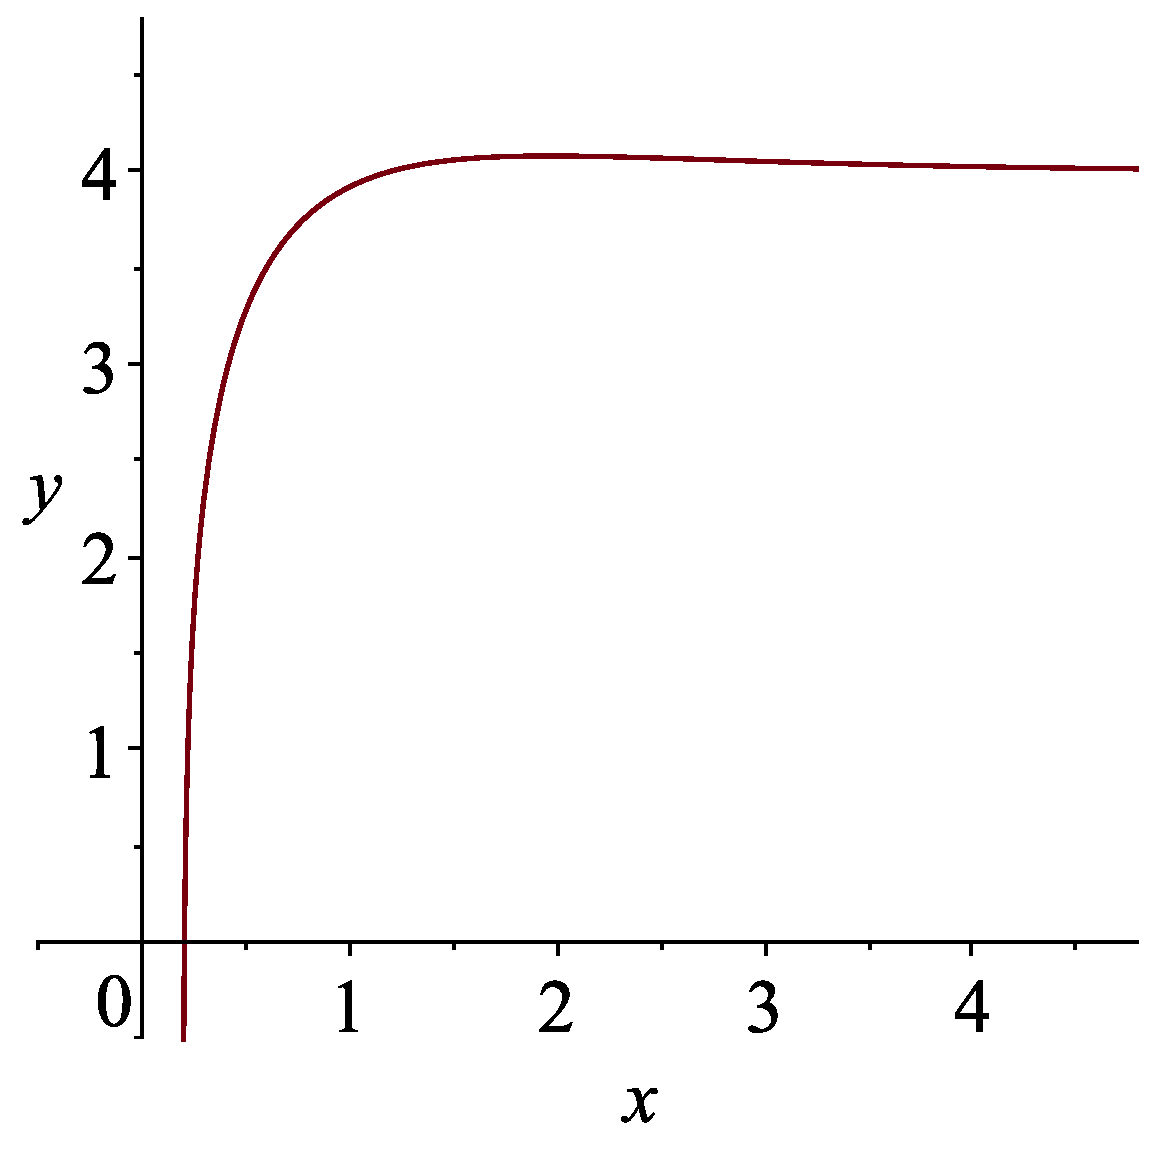
\includegraphics[width=.35 \textwidth]{Curv1.pdf}
\end{image}

This is clearly a pointwise property;  the curve changes direction very quickly at, say $x=1/2$, compared to at $x=3$.

In order to introduce a way to measure this, we make the convention that a line should have zero curvature at each point along it.  To explore how to quantify a change in direction, do the following.


In the figure above, consider the tangent line to the curve at $x=1/2$, $x=1$, $x=3$, and $x=4$.  

\begin{itemize}
\item What do you notice about the relationship of the tangent lines at $x=1/2$ and $x=1$?  

\begin{multipleChoice}
\choice{The tangent lines have similar slopes.}
\choice[correct]{The tangent have very different slopes.}
\end{multipleChoice}

\item What do you notice about the relationship of the tangent lines at $x=3$ and $x=4$? 
\begin{multipleChoice}
\choice[correct]{The tangent lines have similar slopes.}
\choice{The tangent have very different slopes.}
\end{multipleChoice}

\end{itemize}



\begin{exercise}
From the picture, when the curve changes direction quickly, the tangent lines to the curve change quickly.  Thus, a good measure of curvature is to measure the change of the tangent lines.

Since we want to work with curves in space, it is necessary to introduce a parameter to describe the curve.  We thus choose a parameter and describe the curve in the usual way by the position vector $\vec{r}(t)$. A vector parallel to the tangent line is thus $\vec{T}(t) = \vec{r}'(t)$.  In calculus, we like to measure change using derivatives, so can we measure the change by considering the magnitude of how $\vec{T}'(t)$ changes.  There is an important point to consider though.

Consider the ``disguised'' line traced out by $\vec{r} (t) =\vector{t^3,t^3,t^3}$.  

Since this is a line, we want the curvature to be $\answer{0}$.

Now, we can calculate $\vec{r}'(t) = \vector{\answer{3t^2},\answer{3t^2},\answer{3t^2}}$, so $\vec{T}(t) = \vector{\answer{3t^2},\answer{3t^2},\answer{3t^2}}$ and

\[ \vec{T} '(t) = \vector{6t,6t,6t} \]
and thus 

\[\left|\vec{T}'(t)\right| = \answer{3\sqrt{6} t}.\]

So what is the problem?

\begin{exercise}

While it is true that $\vec{T}(t)$ is a vector in the direction of the tangent line, there are two reasons that it can change:

\begin{itemize}
\item The \emph{magnitude} of $\vec{T}(t)$ can change.
\item The \emph{direction} of $\vec{T}(t)$ can change.  
\end{itemize} 
We are not interested in how the magnitude changes; we only are concerned with how the direction changes.  To ensure that the magnitude does not change,  we instead consider the \emph{unit} tangent vector $\uvec{T}(t) = \frac{\vec{T}(t)}{|\vec{T}(t) |}$. Since the magnitude of a unit vector is always $1$, the only way that the vector $\uvec{T}(t)$ can change along the curve is if its direction changes.

Now, consider the line defined by $\vec{r}(t) = \left<t^3,t^3,t^3\right>$ again.  We find that $\left|\vec{T}(t)\right| = \answer{3\sqrt{3}t^2}$, and thus 

\[ \uvec{T}(t) = \frac{\vec{T}(t)}{|\vec{T}(t)|}=\vector{\answer{\frac{1}{\sqrt{3}}}, \answer{\frac{1}{\sqrt{3}}}, \answer{\frac{1}{\sqrt{3}}}}\]

Thus, $\vec{T}'(t) = \vector{\answer{0},\answer{0},\answer{0}}$ and $\left|\vec{T}'(t)\right| = \answer{0}$.

\begin{exercise}

Another important consideration is that we want to ensure that small changes in the parameter we choose results in small changes in the location on the curve.  We can think of the parameter $t$ as a time parameter, and the given parameterization of a curve not only tells us what the curve is, but how quickly it is traced out.  If the curve is being traced out very quickly (for example, consider the curve $x(t) = e^{t}, y(t) = t$ for large values of $t$) small changes in time may produce large distances travelled.  We want to ensure that we are comparing the tangent vector at a given point to a nearby tangent vector.  

One way to ensure that small changes in the input parameter do not yield large distances travelled along the curve is to parametrize the curve by arclength.  With this in mind, we can now define the ``curvature'' as a way to quantify how much the curve changes direction.


\begin{definition}

Let $\vec{r}(s)$ describe a smooth curve parameterized by arclength, and $\uvec{T}(s)$ denote the unit tangent vector.  Then, the \emph{curvature}, denoted by $\kappa$, is the magnitude of the rate of change of the unit tangent vector with respect to arclength.  That is, 

\[ 
\kappa(s) = \left| \frac{d \uvec{T}}{ds} \right|.
\]

\end{definition}


% ADD LATER

%\item[IV.] Consider the helix given by $\left< \frac{3}{2}\cos (t^2),   \frac{3}{2}\sin (t^2),  2t^2 \right>$ for $t \geq 0$.  We will compute the curvature in two ways.
%
%\begin{itemize}
%\item[\underline{Way 1}:] Using arclength as a parameter.
%
%\item[A.] Show that the helix is NOT parameterized by arclength.
%
%\vspace{30mm}
%
%\item[B.] Find a parameterization for the helix in terms of the arclength parameter, $s$.
%
%\newpage
%
%\item[C.] Compute the unit tangent vector $\uvec{T}(s)$; i.e. find $\uvec{T}$ in terms of the arclength parameter, $s$.
%
%\vspace{80mm}
%
%\item[D.] Compute $\kappa(s)$ from $\kappa(s) = \left| \frac{d \uvec{T}(s)}{ds} \right| $.  
%
%\vspace{50mm}
%
%\item[E.] Use the relationship you found between the arclength parameter $s$ and time parameter $t$ in B. to express $\kappa$ in terms of the original time parameter $t$.
   
As we noted earlier, parameterizing a curve by arclength is at best computationally annoying, and sometimes can be impossible!  Integrating square roots can be troublesome; in fact, there are very few expressions involving radicals for which we can compute antiderivatives.  Also, once we find $s$ in terms of $t$, we have to solve for $t$ in terms of $s$, which also may be impossible (for instance, how would you solve $s= t +e^t$ for $t$ in terms of $s$?)

One common theme in multivariable calculus is to use arclength parameterizations to formulate definitions, then use the chain rule to express the results with respect to the original parameter in the problem. 

Since the arclength parameter $s$ is related to the given parameter by 

\[
s = \int^t_0 \left| \vec{r}  '(\tau) \right|  d \tau,\]

We can use the Fundamental Theorem of Calculus to write $\frac{ds}{dt}$ = \wordChoice{\choice{$|\vec{r}'(\tau)|$}\choice[correct]{$|\vec{r}'(t)|$}}.

In the original definition, $\kappa$ is a function of the arclength parameter $s$, but we can think of $\kappa$ as a function of either parameter.  Since we are given the parameter $t$, we want to express the curvature in terms of $t$. 

Using the chain rule

\[ \kappa(t) =  \left| \frac{\d \uvec{T}}{\d s} \right| =  \left| \frac{\d \uvec{T}}{\d t} \cdot \frac{\d t}{\d s} \right| =  \frac{|\d \uvec{T}/ \d t|}{\d s/ \d t} \] 

We just computed $\frac{ds}{dt}$ in terms of $t$ (since $\frac{ds}{dt} = |\vec{r}'(t)|$, which can be computed from the given parameter $t$ without having to find an arclength parameterization), so 

\[ \kappa(t) =  \frac{|d\uvec{T}/dt|}{ \left| \vec{r}  '(t) \right|}. \]

Let's study this in the context of a specific example.  Are you ready?

\begin{multipleChoice}
\choice[correct]{Yes.}
\choice{No.}
\end{multipleChoice}

\begin{exercise}

Consider the helix traced out by $\vec{r}(t) = \vector{\frac{3}{2}\cos (t^2), \frac{3}{2}\sin (t^2), t^2}$ for $t \geq 0$.

\begin{itemize}
\item[1.] Find $\uvec{T}(t)$ (i.e. find $\uvec{T}$ as a function of $t$).

To do this, we compute $\vec{r}'(t)=\vector{ \answer{-3t \sin(t^2)}, \answer{3t \cos(t^2)}, \answer{2t}}$, so $\left|\vec{r}'(t)\right| = \answer{\sqrt{13}t}$, and 

\[
\uvec{T}(t) =\vector{ \answer{\frac{-3 \sin(t^2)}{\sqrt{13}}}, \answer{\frac{3 \cos(t^2)}{\sqrt{13}}}, \answer{\frac{2}{\sqrt{13}}}}
\]
\item[2.] Find $\left|\frac{\d \uvec{T}}{\d t}\right|$.

We find $\uvec{T}'(t) = \vector{ \answer{\frac{-6t \cos(t^2)}{\sqrt{13}}}, \answer{\frac{-6t \sin(t^2)}{\sqrt{13}}}, \answer{0}}$, so 

\[
\left|\frac{\d \uvec{T}}{\d t}\right| = \answer{\frac{6t}{\sqrt{13}}}.
\]

\item[3.] Calculate $\kappa(t)$ using the earlier result.

\[
\kappa(t) = \answer{\frac{6}{13}}.
\]

\begin{feedback}[correct]
In general, this quantity might depend on $t$ (i.e. the direction might change differently at different points on the curve).  Here, we chose a more computationally palatable example to illustrate how to work through the neeccesary calculations.
\end{feedback}
\end{itemize}

\end{exercise}
\end{exercise}
\end{exercise}
\end{exercise}
 \end{exercise}
\end{document}
